\section{Modular Simulation}
\label{sec:approach}
We argue that \emph{end-to-end simulations can be effectively
assembled from multiple different interconnected and synchronized
simulators for individual components.}
%
To demonstrate this, we present \sysname, a new modular simulation
framework that aims to provide end-to-end network system simulation.

\paragraph{End-to-end simulations are better.}
Returning to the dctcp example from earlier, \autoref{fig:dctcp-setup}
shows the simulation setup that produces the result shown in
\autoref{fig:dctcp}.
%
We combine four instances of gem5 with four instances of the Intel
i40e NIC simulator we developed, each pair connected through PCIe;
all NIC simulators are in turn connected to an instance of ns-3.
%
The gem5 instances are running a full Ubuntu image with
unmodified NIC drivers and iperf.
%
\autoref{fig:dctcp} shows that our \sysname simulation approximates
the behavior of the physical testbed much more closely than ns-3, and
yields the same insight.
%
We conclude that end-to-end evaluation with \sysname improves accuracy
for network system evaluation over non-end-to-end simulators.


\subsection{Design Goals}
\label{ssec:approach:goals}
To address the challenges for using simulations in systems research,
(\autoref{ssec:bg:sysresearch}), we have the following design goals
for
\sysname:

\begin{itemize}
  \item \textbf{End-to-end}: simulate full network systems,
    with hosts, existing or custom devices, network topologies, and
    the full software stack, including unmodified OS and applications.
  \item \textbf{Scalable}: simulate large network systems consisting
    of tens or hundreds of separate hosts and devices.
  \item \textbf{Fast}: keep simulation times as low as possible.
  \item \textbf{Modular}: enable flexible composition of simulators, where
    components can be added and swapped independently.
  \item \textbf{Accurate}: preserve accuracy of constituent
    simulators, correctly interface and synchronize components to
    behave equivalent to a monolithic simulator with the same
    models.
  \item \textbf{Deterministic}: keep end-to-end simulation
    deterministic when all individual simulators are deterministic.
  \item \textbf{Transparent}: provide deep and detailed visibility
    into end-to-end performance without affecting simulation behavior,
    to support debugging and performance analysis.
\end{itemize}


\begin{figure}[t]%
\centering%
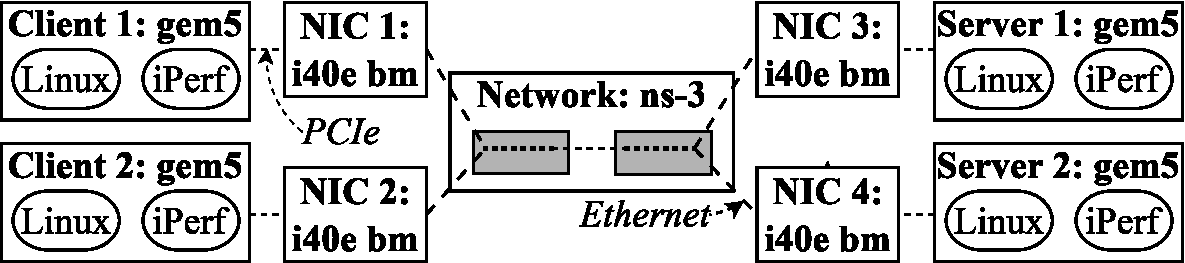
\includegraphics[width=\columnwidth]{figures/dctcp_setup}%
\caption{\sysname configuration for the dctcp experiment in
  \autoref{fig:dctcp}, combining gem5, ns-3, and an Intel NIC
  simulator. Each simulator runs in a separate process.}%
\label{fig:dctcp-setup}%
\Description{Digram with boxes for individual simulators and their
  connections. Starting on the left, two boxes representing separate
  gem-5 instances running Linux and iPerf as the client hosts. These
  connect to a separate next box for an i40e NIC simulator instance
  each. Finally these client NICs connect to a central box that
  represents the ns-3 network simulator. On the right side the
  mirror-image for two server hosts, again with two NICs and two
  servers.}
\end{figure}



\subsection{Technical Challenges}
Achieving our design goals incurs the following challenges:

\paragraph{Simulation interconnection interfaces.}
Unfortunately, existing simulators are standalone and provide no suitable
interfaces for interconnecting with other external simulators.
%
Moreover, enabling modular ``plug-and-play'' configurations, where
components can be independently swapped out, requires common,
well-defined interfaces between different component types.

\paragraph{Scalable synchronization and communication.}
Individual component simulators maintain their own virtual simulation
clocks that progress at different rates.
%
To accurately connect simulators, we need to synchronize their virtual
clocks.
%
However, this synchronization comes at a performance cost, especially
with increasing system scale.
%
For example, we measure a $3.7\times$ increase in runtime for the
dist-gem5~\cite{mohammad:distgem5} simulator when scaling from 2 to 16
simulated hosts, due to synchronization overhead
(\autoref{ssec:eval:syncproto}).
%
Prior work shows synchronization overhead can be reduced by
sacrificing accuracy and determinism through lax synchronization.
\cite{fujimoto:relaxedsim,chen:slacksim}.
%
Since this violates two of our design goals, we do not consider this.

\paragraph{Incompatible simulation models.}
Finally, different simulators often employ mutually incompatible
simulation models.
%
For example, QEMU has a synchronous device model where calls in device
code block until complete, while ns-3 schedules asynchronous events
to model networks, and Verilator simulates hardware circuits cycle by
cycle.
%
We therefore need an interface compatible with all of these simulation
models.

\subsection{Design Principles}
We address these challenges through four design principles:

\paragraph{Fix natural component simulator interfaces.}
To enable modular composition of simulators, \sysname defines an
interface for each \textit{component type}
(\autoref{ssec:design:interface}).
%
We base these interfaces on the \emph{point-to-point} component
boundaries in real systems:
PCI express (PCIe) connects today's hardware devices to servers, while
network devices typically connect through Ethernet networks.
%
We choose these interfaces as a starting point, but our approach
generalizes to other interconnects and networks.
%
These component interfaces form narrow waists, decoupling innovation on
both sides:
%
To integrate a simulator into \sysname, developers need to add an
adapter that implements the component interface, without needing to
modify other simulators.
%
We assume a static topology of components throughout a simulation.


\paragraph{Loose coupling with message passing.}
Instead of tightly integrating multiple simulators into one simulation
loop, \sysname runs component simulators as separate processes that
communicate through message passing (\autoref{ssec:design:interface})
across our defined interfaces.
%
This drastically simplifies integrating simulators into \sysname,
as we treat each simulator as a black-box that only needs to
implement our interfaces.
%
Using asynchronous message passing also maximizes compatibility with
different simulation models:
%
Discrete event and cycle-by-cycle simulations can issue requests and
process responses at the scheduled times, while blocking simulations
can block till the response message arrives --- for peer simulators
this is transparent.
%
Message passing channels also provide inspection points for debugging
and tracing system behavior without modifying component simulators.


\paragraph{Parallel execution with shared memory queues.}
We run simulators in parallel on different host cores and connect them
through optimized shared-memory queues
(\autoref{ssec:design:transport}).
%
As simulators run on separate cores and only communicate when
necessary, this avoids unnecessary cache-coherence traffic and
hidden scalability bottlenecks.
%
These mechanisms allow us to
(i) \textit{scale up} to large simulations: Instead of simulating the
complete system in one simulation instance, we simulate different
components of the system in separate simulators running in parallel
(\autoref{ssec:design:decomp}).
%
(ii) \textit{scale out} with distributed simulations: We use a
separate proxy that transparently forwards messages on shared memory
queues over the network to and from simulators running on remote hosts
(\autoref{ssec:design:proxy}).



\paragraph{Accurate and efficient synchronization.}
We ensure accurate simulation through correct time synchronization among
simulators, but with minimum runtime overhead.
%
\emph{Synchronization is optional}, and the user can disable it for
unsynchronized emulations.
%
For this, we combine three key insights:
%
1)~\emph{Global synchronization is not necessary} as our simulator
boundaries at point-to-point interfaces limit which simulators
directly communicate.
%
As long as events at these pairwise interfaces are processed in a
time-synchronized manner, simulation behavior is correct.
%
2)~\emph{Latency at component interfaces provides slack}, reducing
frequency of component having to wait for others to
coordinate~\cite{chen:slacksim} and thus synchronization overhead.
%
An event sent at time $T$ only arrives at $T+\Delta$, as our component
interfaces have an inherent latency $\Delta$ in physical systems that
we model.
%
3)~By \emph{inlining synchronization with efficient polled
message transfers}, synchronization overheads can be minimized and
sometimes completely avoided.
%
We combine these observations to design an accurate, efficient, and
scalable synchronization mechanism for parallel end-to-end simulations
(\autoref{ssec:design:syncproto}).



\subsection{Non-Goals}
\sysname is not a panacea. We explicitly view the following aspects as
out of scope for this paper and leave them for future work:

\paragraph{Accelerating component simulators.} \sysname does not
generally aim to reduce simulation times for individual component
simulators as we only modify simulators to add \sysname adapters.
%
Simulation times for synchronized end-to-end \sysname simulations are
at least as high as the slowest component simulator, and may increase
due to synchronization and communication overhead.
%
However, in a few cases, \sysname interfaces enable developers to
decompose an existing component simulator into multiple smaller
parallel pieces, thereby reducing simulation time
(\autoref{ssec:eval:decomp}).

\paragraph{Avoiding need for validation.}
To obtain representative results, users need to validate component
simulation configurations in \sysname as with any other simulation.
%
Validation effort is no higher in \sysname than it would be in an
equivalent monolithic simulator, as \sysname forwards timestamped
events accurately from one simulator-internal interface to another
without modifying them (except for the configured link latency).
%
We expect, however, that \sysname could reduce validation effort by
allowing users to re-combine validated component simulator
configurations without validating from scratch.
(\autoref{sec:discussion})

\paragraph{Interfacing semantically incompatible simulators.}
While \sysname can combine simulators that use different models for
simulation, it cannot bridge semantic gaps between simulators.
%
For example, \sysname cannot connect a gem5 host sending packets
through an RTL NIC with a flow-based network simulator.
%
Such conversions may be possible in special cases, but are specific to
the concrete simulators, and as such could be integrated as part of a
\sysname adapter in such a simulator.
